\chapter{牙齿与合理饮食}\label{ch:g2:teeth-and-eating-well}

咬一口苹果，看看上面的痕迹：整齐弯曲的一排
小印子。这是你的牙齿留下的——一整套工具箱，能切、能撕、能磨，
每一餐在咽下之前都要经过它们。像每一套好工具一样，
它值得好好保养，也需要好好使用。

\begin{omfigure}
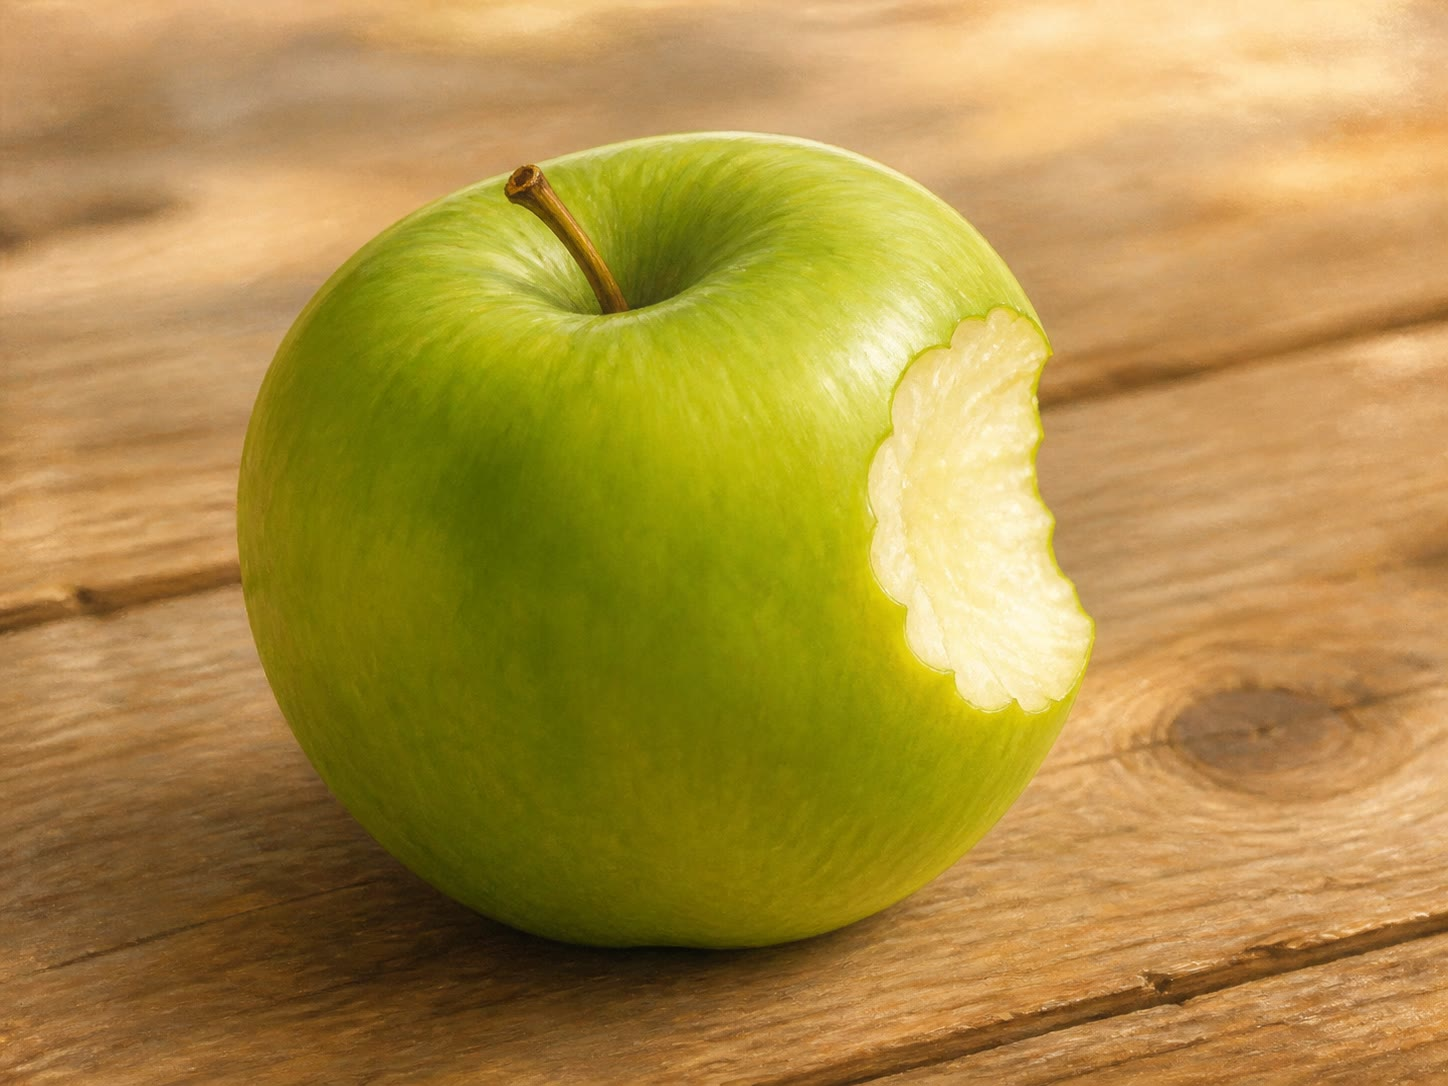
\includegraphics[width=0.55\linewidth]{images/book1/ai/g2-teeth-apple.jpg}

{\small 本章的第一件“展品”：咬一口，\omterm{def:g2:teeth-and-eating-well:kinds}{门齿}留下的
整齐弯曲的印记。}
\end{omfigure}

\section{牙齿：口腔里的工具箱}

\begin{definition}[人的三种牙齿]\label{def:g2:teeth-and-eating-well:kinds}
人的牙齿分为三种，各有各的作用：
\begin{enumerate}
  \item \emph{门齿}\index{门齿}，位于前部，扁平而锋利，
        \emph{切}——负责切开苹果；
  \item \emph{犬齿}\index{犬齿}，尖尖的，位于嘴角，
        \emph{撕}——用来咬住并拉扯较硬的食物；
  \item \emph{臼齿}\index{臼齿}，宽大而凹凸不平，位于后部，
        \emph{磨}——把食物磨碎成糊状，
        便于咽下。
\end{enumerate}
\end{definition}

\begin{omfigure}
\begin{tikzpicture}
  \node[anchor=south west, inner sep=0] (img) at (0,0)
    {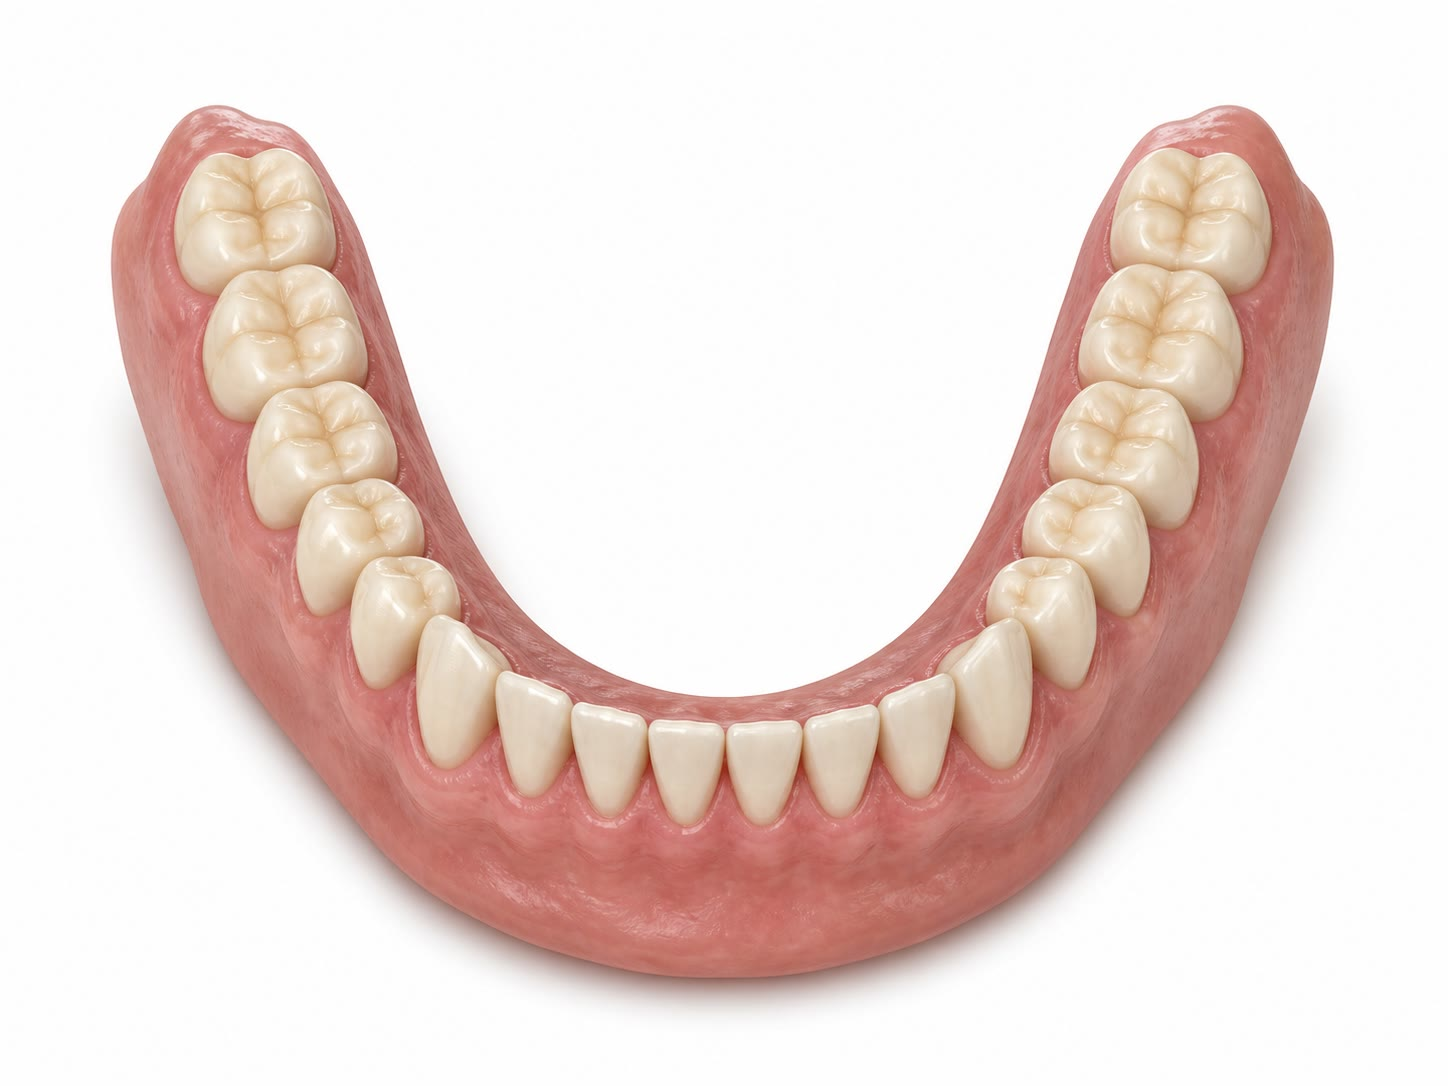
\includegraphics[width=0.56\linewidth]{images/book1/ai/fig-jaw-teeth.jpg}};
  \begin{scope}[x={(img.south east)}, y={(img.north west)},
      every node/.style={font=\small}]
    \draw[omDef, thick] (0.50,0.28) -- (0.50,0.06)
      node[below] {门齿：切};
    \draw[omThm, thick] (0.31,0.44) -- (-0.03,0.40)
      node[left, align=right, omThm] {犬齿：\\ 撕};
    \draw[omMeth, thick] (0.80,0.72) -- (1.03,0.72)
      node[right, align=left, omMeth] {臼齿：\\ 磨};
  \end{scope}
\end{tikzpicture}

{\small 下颌：前部的\omterm{def:g2:teeth-and-eating-well:kinds}{门齿}负责切，
\omterm{def:g2:teeth-and-eating-well:kinds}{犬齿}位于嘴角负责撕，后部的\omterm{def:g2:teeth-and-eating-well:kinds}{臼齿}负责磨。}
\end{omfigure}

\begin{example}[咬一口苹果，三种工具]\label{ex:g2:teeth-and-eating-well:apple}
吃一块苹果，要按顺序用上整个工具箱：
\omterm{def:g2:teeth-and-eating-well:kinds}{门齿}先切下一口，\omterm{def:g2:teeth-and-eating-well:kinds}{犬齿}帮忙把它拉下来，
然后舌头把食物送到\omterm{def:g2:teeth-and-eating-well:kinds}{臼齿}处，由\omterm{def:g2:teeth-and-eating-well:kinds}{臼齿}磨碎。
最后才咽下。
\end{example}

\begin{remark}[想一想动物]\label{rem:g2:teeth-and-eating-well:animals}
你的这套混合工具箱有个道理：扁平的切割与研磨工具像
\omterm{def:g2:what-animals-eat:kinds}{植食性动物}，尖尖的\omterm{def:g2:teeth-and-eating-well:kinds}{犬齿}像\omterm{def:g2:what-animals-eat:kinds}{肉食性动物}。
这是\omterm{def:g2:what-animals-eat:kinds}{杂食性动物}的口腔——人的牙齿既适合吃\omterm{def:g1:plants-around-us:plant}{植物}，\emph{也}适合吃肉，
正如\cref{ch:g2:what-animals-eat}把我们归了类。
\end{remark}

\section{乳牙与恒牙}

\begin{proposition}[一生两副牙齿]\label{prop:g2:teeth-and-eating-well:sets}
人一生会长出两副牙齿。$20$ 颗\emph{乳牙}\index{乳牙}
在生命最初几年陆续长出。
大约六岁起开始松动，一颗颗脱落，
由下方的\emph{恒牙}\index{恒牙}向上推挤。\omterm{prop:g2:teeth-and-eating-well:sets}{恒牙}是最后一副，
最多 $32$ 颗，要用上一辈子。
\end{proposition}
\admitted

\begin{example}[松动的门齿]\label{ex:g2:teeth-and-eating-well:wobbly}
一颗前\omterm{def:g2:teeth-and-eating-well:kinds}{门齿}在孩子刚上学的年纪开始松动。
在它下面，一颗\omterm{prop:g2:teeth-and-eating-well:sets}{恒牙}\omterm{def:g2:teeth-and-eating-well:kinds}{门齿}一直在悄悄生长，
慢慢溶解\omterm{prop:g2:teeth-and-eating-well:sets}{乳牙}的牙根，直到小牙脱落。
缺口并非偶然，而是一次更替。
\end{example}

\begin{remark}[没有第三副牙]\label{rem:g2:teeth-and-eating-well:nothird}
\omterm{prop:g2:teeth-and-eating-well:sets}{恒牙}之后不会再有新牙。\omterm{prop:g2:teeth-and-eating-well:sets}{乳牙}掉了会被替换，
\omterm{prop:g2:teeth-and-eating-well:sets}{恒牙}掉了就没有了。这才是大人一再叮嘱刷牙的真正原因：
第二套工具箱要用好，要撑过
七十年或更久。
\end{remark}

\section{合理饮食}

\begin{proposition}[均衡的餐盘]\label{prop:g2:teeth-and-eating-well:balanced}
要长身体、保持健康，身体每天都需要各类食物，
每天都要吃够。
\begin{itemize}
  \item 水果和蔬菜——补充维生素，每餐都要吃；
  \item 面包、谷类、土豆——提供持久的能量；
  \item \omterm{def:g2:animals-grow-up:born}{乳汁}、酸奶、奶酪——帮助长骨骼和牙齿；
  \item 肉、鱼类或卵——用来构建身体，每天
        吃一到两次就够了；
  \item 水——身体真正需要的唯一饮品；
  \item 含糖、高脂的零食——图个口福，
        只能少量吃，不要每餐都吃。
\end{itemize}
\end{proposition}
\admitted

\begin{example}[两袋零食]\label{ex:g2:teeth-and-eating-well:snack}
零食 A：一个苹果、一片面包、一杯水。零食 B：糖果、
一瓶汽水。零食 B 尝起来只有糖味，几乎别无他味——而糖正是
正是\cref{ch:g1:healthy-habits}中\omterm{def:g1:healthy-habits:germs}{病菌}最爱吃的东西。
零食 A 滋养身体，也让牙齿得到实实在在的锻炼。猜猜看，
牙医给自己孩子装的是哪一袋？
\end{example}

\begin{method}[检查一天的菜单]\label{met:g2:teeth-and-eating-well:check}
回顾一天的三餐，检查以下几点：
\begin{enumerate}
  \item 每餐是否都有水果或蔬菜？
  \item 是否有食物类别中的食物——奶制品，以及肉、
        鱼或卵？
  \item 是否把水作为日常饮品？
  \item 零食是否少量，且只偶尔吃？
\end{enumerate}
若缺少某一类食物，下一餐正是把它
请回餐桌的机会。
\end{method}

\section{练习}

\begin{exercise}[$\star$]\label{exo:g2:teeth-and-eating-well:1}
说出三类牙齿及各自的作用。
\end{exercise}

\begin{exercise}[$\star$]\label{exo:g2:teeth-and-eating-well:2}
哪些牙齿在口腔前部，哪些在后部？
\end{exercise}

\begin{exercise}[$\star$]\label{exo:g2:teeth-and-eating-well:3}
跟随一口胡萝卜穿过口腔，
按顺序说出各种牙齿分别做什么？
\end{exercise}

\begin{exercise}[$\star$]\label{exo:g2:teeth-and-eating-well:4}
\omterm{prop:g2:teeth-and-eating-well:sets}{乳牙}有多少颗？从大约
六岁起，它们会发生什么变化？
\end{exercise}

\begin{exercise}[$\star$]\label{exo:g2:teeth-and-eating-well:5}
为什么\omterm{prop:g2:teeth-and-eating-well:sets}{恒牙}比\omterm{prop:g2:teeth-and-eating-well:sets}{乳牙}更需要细心保护？
\end{exercise}

\begin{exercise}[$\star$]\label{exo:g2:teeth-and-eating-well:6}
说出健康的一天应包括的食物类别，
以及身体真正需要的是哪一种饮料？
\end{exercise}

\begin{exercise}[$\star$]\label{exo:g2:teeth-and-eating-well:7}
比较\cref{ex:g2:teeth-and-eating-well:snack}中的两袋零食：
零食 A 给身体带来什么是零食 B 没有的？
\end{exercise}

\begin{exercise}[$\star$]\label{exo:g2:teeth-and-eating-well:8}
试一试：对着镜子看看自己的牙齿，找出一颗\omterm{def:g2:teeth-and-eating-well:kinds}{门齿}、
一颗\omterm{def:g2:teeth-and-eating-well:kinds}{犬齿}和一颗\omterm{def:g2:teeth-and-eating-well:kinds}{臼齿}，对照图形检查它们的形状。
\end{exercise}

\begin{exercise}[$\star\star$]\label{exo:g2:teeth-and-eating-well:9}
利用\cref{rem:g2:teeth-and-eating-well:animals}，说明
人类牙齿的形状反映了人类的食物构成——并指出
\cref{ch:g2:what-animals-eat}中哪些\omterm{def:g1:animals-around-us:animal}{动物}与人类相似。
\end{exercise}

\begin{exercise}[$\star\star$]\label{exo:g2:teeth-and-eating-well:10}
莉拉的一天：早餐——麦片和\omterm{def:g2:animals-grow-up:born}{乳汁}；午餐——意大利面和
糖果；加餐——汽水和饼干；晚餐——披萨。用
\cref{met:g2:teeth-and-eating-well:check}检查这一天：
缺少了什么，哪些出现得太频繁？
\end{exercise}
